\documentclass[11pt]{article}
\usepackage[utf8]{inputenc}
\usepackage[T1]{fontenc}
\usepackage{amsmath}
\usepackage{amssymb}
\usepackage{multicol}
\usepackage{geometry}
\usepackage{tikz}
\usepackage{enumitem}
\usepackage{xcolor}
\usepackage{titlesec}

% Configurações de layout
\geometry{a4paper, left=1cm, right=1cm, top=0.5cm, bottom=1.2cm}
\setlength{\columnseprule}{0.4pt}

% Cores para títulos
\titleformat{\section}{\normalfont\Large\bfseries\color{blue}}{\thesection}{1em}{}
\titleformat{\subsection}{\normalfont\large\bfseries\color{red}}{\thesubsection}{1em}{}

\title{\textcolor{green}{Primeiro Trimestre: Matemática
    \\Introdução à Estatística}}
\author{Professor: Jefferson}
\date{}

\begin{document}

\maketitle
\vspace{-1cm}

%\begin{center}
%\large{Nome: \underline{\hspace{8cm}} \quad Turma: \underline{\hspace{3cm}}}
%\end{center}

\begin{multicols}{2}

\section*{O que é Estatística?}

\textbf{Estatística} é a ciência que coleta, organiza, analisa e interpreta dados para tomar decisões.

\subsection*{Aplicações no dia a dia}
\begin{itemize}
\item Pesquisas de opinião
\item Controle de qualidade
\item Previsões meteorológicas
\item Análise de desempenho esportivo
\item Indicadores econômicos
\end{itemize}

\section*{Conceitos Fundamentais}

\subsection*{População e Amostra}

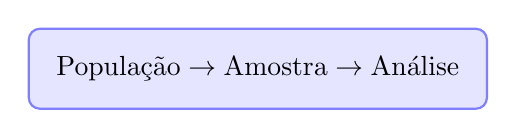
\begin{tikzpicture}
\node[rectangle, fill=blue!10, rounded corners, inner sep=10pt, draw=blue!50, thick] (box) {
$\displaystyle \text{População} \rightarrow \text{Amostra} \rightarrow \text{Análise}$
};
\end{tikzpicture}

\textbf{Definições:}
\begin{itemize}
\item \textbf{População}: Conjunto total de elementos estudados
\item \textbf{Amostra}: Parte representativa da população
\item \textbf{Censo}: Estudo de toda a população
\end{itemize}

\subsection*{Variáveis Estatísticas}

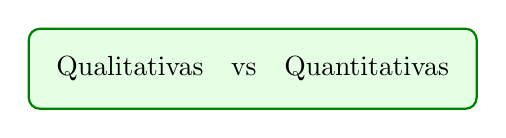
\begin{tikzpicture}
\node[rectangle, fill=green!10, rounded corners, inner sep=10pt, draw=green!50!black, thick] (box) {
$\displaystyle \text{Qualitativas} \quad \text{vs} \quad \text{Quantitativas}$
};
\end{tikzpicture}

\textbf{Tipos de variáveis:}
\begin{itemize}
\item \textbf{Qualitativas}: Descrevem qualidade (cor, gênero)
  \begin{itemize}
  \item Nominais: sem ordem (estado civil)
  \item Ordinais: com ordem (escolaridade)
  \end{itemize}
\item \textbf{Quantitativas}: Expressam quantidade
  \begin{itemize}
  \item Discretas: valores inteiros (número de filhos)
  \item Contínuas: quaisquer valores (altura, peso)
  \end{itemize}
\end{itemize}

\section*{Organização de Dados}

\subsection*{Tabelas de Frequência}

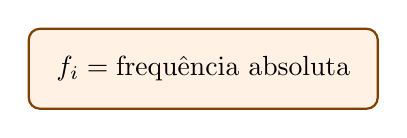
\begin{tikzpicture}
\node[rectangle, fill=orange!10, rounded corners, inner sep=10pt, draw=orange!50!black, thick] (box) {
$\displaystyle f_i = \text{frequência absoluta}$
};
\end{tikzpicture}

\textbf{Tipos de frequência:}
\begin{itemize}
\item \textbf{Absoluta} ($f_i$): Número de ocorrências
\item \textbf{Relativa} ($fr_i$): $fr_i = \frac{f_i}{n}$
\item \textbf{Percentual}: $fr_i \times 100\%$
\item \textbf{Acumulada}: Soma das frequências
\end{itemize}

\subsection*{Gráficos Estatísticos}

\textbf{Principais tipos:}
\begin{enumerate}
\item \textbf{Gráfico de colunas/barras}
\item \textbf{Histograma} (dados contínuos)
\item \textbf{Gráfico de setores} (pizza)
\item \textbf{Polígono de frequência}
\item \textbf{Ogiva} (frequência acumulada)
\end{enumerate}

\section*{Medidas de Posição}

\subsection*{Média Aritmética}

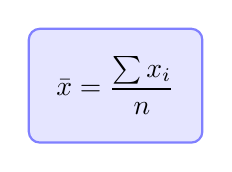
\begin{tikzpicture}
\node[rectangle, fill=blue!10, rounded corners, inner sep=10pt, draw=blue!50, thick] (box) {
$\displaystyle \bar{x} = \frac{\sum x_i}{n}$
};
\end{tikzpicture}

\subsection*{Mediana}

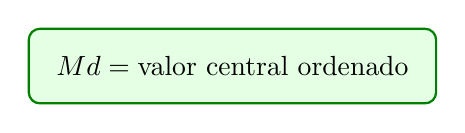
\begin{tikzpicture}
\node[rectangle, fill=green!10, rounded corners, inner sep=10pt, draw=green!50!black, thick] (box) {
$\displaystyle Md = \text{valor central ordenado}$
};
\end{tikzpicture}

\subsection*{Moda}

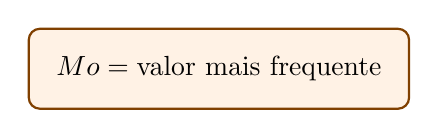
\begin{tikzpicture}
\node[rectangle, fill=orange!10, rounded corners, inner sep=10pt, draw=orange!50!black, thick] (box) {
$\displaystyle Mo = \text{valor mais frequente}$
};
\end{tikzpicture}

\section*{Exercícios Básicos}

\begin{enumerate}[leftmargin=*]

\item Classifique as variáveis:
\begin{enumerate}[label=\alph*)]
\item Número de irmãos
\item Cor dos olhos
\item Temperatura corporal
\item Nível de satisfação (bom, regular, ruim)
\item Salário mensal
\item Marca de celular
\end{enumerate}

\item Dados as idades: 18, 20, 22, 18, 25, 20, 18, 22
\begin{enumerate}[label=\alph*)]
\item Construa a tabela de frequência
\item Calcule frequência relativa
\item Qual a moda?
\end{enumerate}

\item As notas de 10 alunos foram:
\[
5, 6, 7, 8, 5, 6, 9, 7, 6, 8
\]
\begin{enumerate}[label=\alph*)]
\item Calcule a média
\item Encontre a mediana
\item Determine a moda
\end{enumerate}

\item Complete a tabela:
\begin{center}
\begin{tabular}{|c|c|c|c|}
\hline
\textbf{Notas} & \textbf{$f_i$} & \textbf{$fr_i$} & \textbf{\%} \\
\hline
0-2 & 3 & & \\
2-4 & 5 & & \\
4-6 & 8 & & \\
6-8 & 10 & & \\
8-10 & 4 & & \\
\hline
Total & 30 & & \\
\hline
\end{tabular}
\end{center}

\item Problemas contextualizados:
\begin{enumerate}[label=\alph*)]
\item Em uma pesquisa com 50 pessoas sobre time de futebol:
  32 torcem para o time A, 12 para o time B e 6 para o time C.
  Construa o gráfico de setores.
\item As temperaturas máximas de uma semana foram:
  28°, 30°, 29°, 31°, 32°, 30°, 29°C.
  Calcule a temperatura média.
\end{enumerate}

\item Analise o histograma (dados fictícios):
\begin{center}
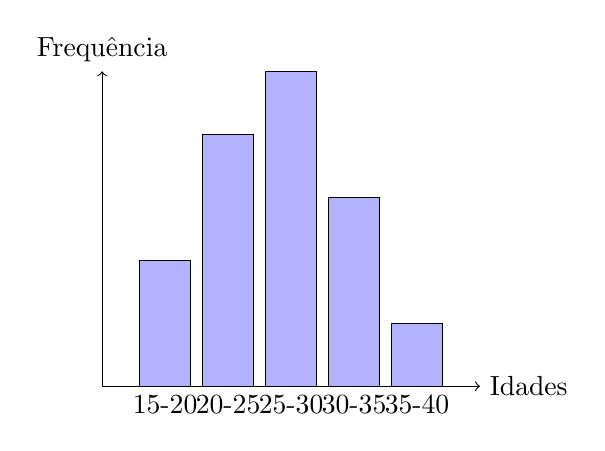
\begin{tikzpicture}[scale=0.8]
\draw[->] (0,0) -- (6,0) node[right] {Idades};
\draw[->] (0,0) -- (0,5) node[above] {Frequência};
\foreach \x/\y in {1/2, 2/4, 3/5, 4/3, 5/1}
  \draw[fill=blue!30] (\x-0.4,0) rectangle (\x+0.4,\y);
\node at (1,0) [below] {15-20};
\node at (2,0) [below] {20-25};
\node at (3,0) [below] {25-30};
\node at (4,0) [below] {30-35};
\node at (5,0) [below] {35-40};
\end{tikzpicture}
\end{center}
\begin{enumerate}[label=\alph*)]
\item Qual faixa etária tem maior frequência?
\item Quantas pessoas têm entre 25 e 30 anos?
\item Qual o total de pessoas pesquisadas?
\end{enumerate}

\item Dados agrupados:
\begin{center}
\begin{tabular}{|c|c|}
\hline
\textbf{Salário (R\$)} & \textbf{Nº funcionários} \\
\hline
1000-1500 & 8 \\
1500-2000 & 12 \\
2000-2500 & 15 \\
2500-3000 & 10 \\
3000-3500 & 5 \\
\hline
\end{tabular}
\end{center}
\begin{enumerate}[label=\alph*)]
\item Calcule o ponto médio de cada classe
\item Calcule a média aproximada
\item Em qual classe está a mediana?
\end{enumerate}

\item Escolha o gráfico adequado:
\begin{enumerate}[label=\alph*)]
\item Distribuição de idade em uma população
\item Preferência por marcas de refrigerante
\item Evolução das vendas ao longo do ano
\item Composição do orçamento familiar
\end{enumerate}

\item Pesquisa sobre meio de transporte:
\begin{center}
\begin{tabular}{|l|c|}
\hline
\textbf{Transporte} & \textbf{Frequência} \\
\hline
Ônibus & 25 \\
Carro & 15 \\
Metrô & 20 \\
Bicicleta & 8 \\
A pé & 12 \\
\hline
Total & 80 \\
\hline
\end{tabular}
\end{center}
\begin{enumerate}[label=\alph*)]
\item Calcule as frequências relativas
\item Construa o gráfico de barras
\item Qual a porcentagem que usa carro?
\end{enumerate}

\item Para cada situação, indique se é população ou amostra:
\begin{enumerate}[label=\alph*)]
\item Todos os alunos da escola
\item 50 clientes sorteados de um supermercado
\item Todas as casas do bairro
\item 1000 eleitores pesquisados
\end{enumerate}

\end{enumerate}

\section*{Exercícios Avançados}

\begin{enumerate}[leftmargin=*, start=11]

\item Duas turmas têm as seguintes médias:
\begin{itemize}
\item Turma A: $\bar{x} = 7,2$ com 30 alunos
\item Turma B: $\bar{x} = 6,8$ com 25 alunos
\end{itemize}
Qual a média geral das duas turmas juntas?

\item Construa a ogiva para os dados:
\begin{center}
\begin{tabular}{|c|c|}
\hline
\textbf{Classes} & \textbf{$f_i$} \\
\hline
10-20 & 4 \\
20-30 & 8 \\
30-40 & 12 \\
40-50 & 10 \\
50-60 & 6 \\
\hline
\end{tabular}
\end{center}

\item Analise criticamente:
\begin{enumerate}[label=\alph*)]
\item "A média salarial da empresa é R\$ 5000"
  (salários: R\$ 2000, 3000, 4000, 15000)
\item Em uma pesquisa, 80\% disseram preferir produto X
  (amostra: 10 pessoas no shopping)
\end{enumerate}

\end{enumerate}

\section*{Dicas para Resolver}

\begin{itemize}
\item \textbf{População vs Amostra}: Censo estuda todos, pesquisa estuda parte
\item \textbf{Variáveis}: Qualitativa descreve, quantitativa mede
\item \textbf{Tabelas}: Organize dados antes de calcular
\item \textbf{Gráficos}: Escolha o tipo conforme os dados
\item \textbf{Média}: Sensível a valores extremos
\item \textbf{Mediana}: Boa para distribuições assimétricas
\item \textbf{Moda}: Útil para dados qualitativos
\end{itemize}

\section*{Projeto Prático}

\textbf{Pesquisa na sala de aula:}
\begin{enumerate}
\item Escolha um tema (esporte favorito, horas de estudo etc.)
\item Colete dados dos colegas
\item Organize em tabela de frequência
\item Calcule medidas de posição
\item Construa um gráfico adequado
\item Interprete os resultados
\end{enumerate}

\end{multicols}

\end{document}
